\setlength\parindent{0pt}
\setcounter{page}{75} 
\begin{figure}[bh]
   	\noindent\centering{
   		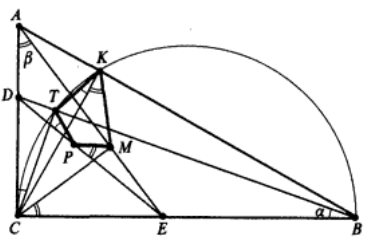
\includegraphics[width=70mm]{photo1.png}
   	}
\end{figure}
\textit{Рис. 14.}
\vspace*{8pt}

нику BCD. Тогда исходный треугольник ABC окажется разрезанным на $k^2$ + $l^2$ = n равных треугольников

1 0 к л а с с

1. Простейший пример $6\cdot1$,  $6\cdot2$,  $6\cdot3$. В общем виде рассмотрите прогрессию A, 2A, ..., (2n - 1)A, где A = $1 \cdot 2 \cdot 3 \cdot$ ... $\cdot (2n - 1)$.

2. Меняя местами число 1 с другими числами, мы можем продвинуть 1 к числу 2. Далее можно двойными шагами (сначала перемещается число 2, затем - число 1) придвинуть пару 1, 2 к числу 3. Теперь тройку 1, 2,3 можно тройными шагами придвинуть к числу 4. И так далее. В итоге придем к естественному (монотонному) упорядочению данных чисел ( по часовой стрелке или против часовой стрелки).

3. Обозначим через K, M, P, T (рис. 14) основания высот, опущенных из точки C на прямые AB, AE, DE и BD соответственно. Ясно, что лучи CK и CP лежат между лучами CT и CM и четырехугольник KMPT является выпуклым. Поэтому, в силу теоремы о вписанном угле, для доказательства утверждения задачи достаточно показать, что $\angle TKM$ + $\angle MPT$ = $180^{\circ}$. Пусть $\alpha$ = $\angle DBC$, $\beta$ = $\angle EAC$. Очевидно, $\angle DCT$ = $\alpha$ (напомним, что $CT \perp DB$) и $\angle MCE$ = $\beta$. Четыре точки C, T, K, B лежат на одной окружности, поскольку углы $\angle CTB$

\begin{table}[h]
    \centering
    \begin{tabular}{|c|c|c|c|c|c|c|c|}
\hline
60 & 59 & 52 & 51 & 44 & 43 & 16 & 15 \\ \hline
61 & 58 & 53 & 50 & 45 & 42 & 17 & 14 \\ \hline
62 & 57 & 54 & 49 & 46 & 41 & 18 & 13 \\ \hline
63 & 56 & 55 & 48 & 47 & 40 & 19 & 12 \\ \hline
64 & 35 & 36 & 37 & 38 & 39 & 20 & 11 \\ \hline
33 & 34 & 29 & 28 & 25 & 24 & 21 & 10 \\ \hline
32 & 31 & 30 & 27 & 26 & 23 & 22 & 9  \\ \hline
1  & 2  & 3  & 4  & 5  & 6  & 7  & 8  \\ \hline
\end{tabular}
\end{table}

\textit{Рис. 15.}



\begin{figure}[h]
    \noindent\centering{
        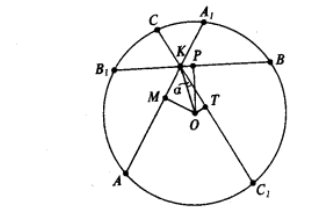
\includegraphics[width=70mm]{photo2.png}
    }
\end{figure}
\textit{Рис. 16}
\vspace*{8pt}

к $\angle CKB$ прямые. Поэтому $\angle TKC$ = $\angle TBC$ = $\alpha$ (эти углы равны как опирающиеся на одну и ту же дугу). Аналогично, $\angle CKM$ = $\angle CAM$ = $\beta$ (точки C, M, K, A лежат на одной окружности), $\angle DPT$ = $\angle DCT$ = $\alpha$ (точки C, P, T, D лежат на одной окружности), $\angle EPM$ = $\angle ECM$ = $\beta$ (точки E, M, P, C лежат на одной окружности). Следовательно, $\angle TKM$ + $\angle TPM$ = ($\alpha$ + $\beta$) + ($180^{\circ}$ - $\alpha$ - $\beta$) = $180^{\circ}$. Отсюда следует требуемое утверждение.

4. Из неравенства между средним арифметическим и средним геометрическим каждое их отношений {\large $\frac{a}{1+a^2}$, $\frac{b}{1+b^2}$, $\frac{c}{1+c^2}$}, не превосходит 1/2. Отсюда следует левое неравенство. Докажем правое неравенство на x, y, z и сложив получающиеся при этом три неравенства, получим неравенство

\[
(1 + $\frac{y}{x}$ + $\frac{z}{x}$) + ($\frac{x}{y}$ + 1 + $\frac{z}{y}$) + ($\frac{x}{z}$ + $\frac{y}{z}$ + 1) \leq 6($\frac{1}{x}$ + $\frac{1}{y}$ + $\frac{1}{z}$),
\]

откуда и следует требуемое неравенство, так как

\[
    \frac{x}{y} + \frac{y}{x} \leq 2, \frac{y}{z} + \frac{z}{y} \leq 2, \frac{z}{x} + \frac{x}{z} \leq 2
\]

5. Указание: рассмотрите график функции y=f(x), где f(x)=($x^2$ - 1)($x^2$ - 10). При c=0 уравнение f(x)=0 имеет только три целых корня (-1, 0 и 1). При c \neq уравнение f(x) = c вне отрезка [-1;1] имеет не более трех корней, а на отрезку [-1;1] целых корней не имеет.

6. a) Не может. Для того чтобы вернуться на поле a1, нужно сделать четное число ходов по горизонтали и четное число ходов по вертикали, т. е. общее число ходов должно быть четным. Число посещений всех полей шахматной доски по условию задачи равно 1 + 2 + 3 +...+64=2080 и является четным. В начальный момент ладья уже находится на поле a1 (есть одно посещение). Следовательно, остается осуществить 2079 посещений и сделать это надо за четное число ходов, что, очевидно, невозможно
